\documentclass{article}

\usepackage{graphicx}
\usepackage{fancyhdr}
\usepackage{enumitem}
\usepackage{caption}
\usepackage{float}
\pagestyle{fancy}

\begin{document}
	\begin{titlepage}
		\begin{center}
			\line(1,0){340}\\
			[0.25in]
			\huge\bfseries Temperature Data Aggregation in Bliss Hall at SUNY New Paltz\\
			[2mm]
			\line(1,0){340}\\
			[1.1cm]
			\textsc{\Large Embedded Linux (CPS342)\\ April 25, 2016}\\
			[1cm]
			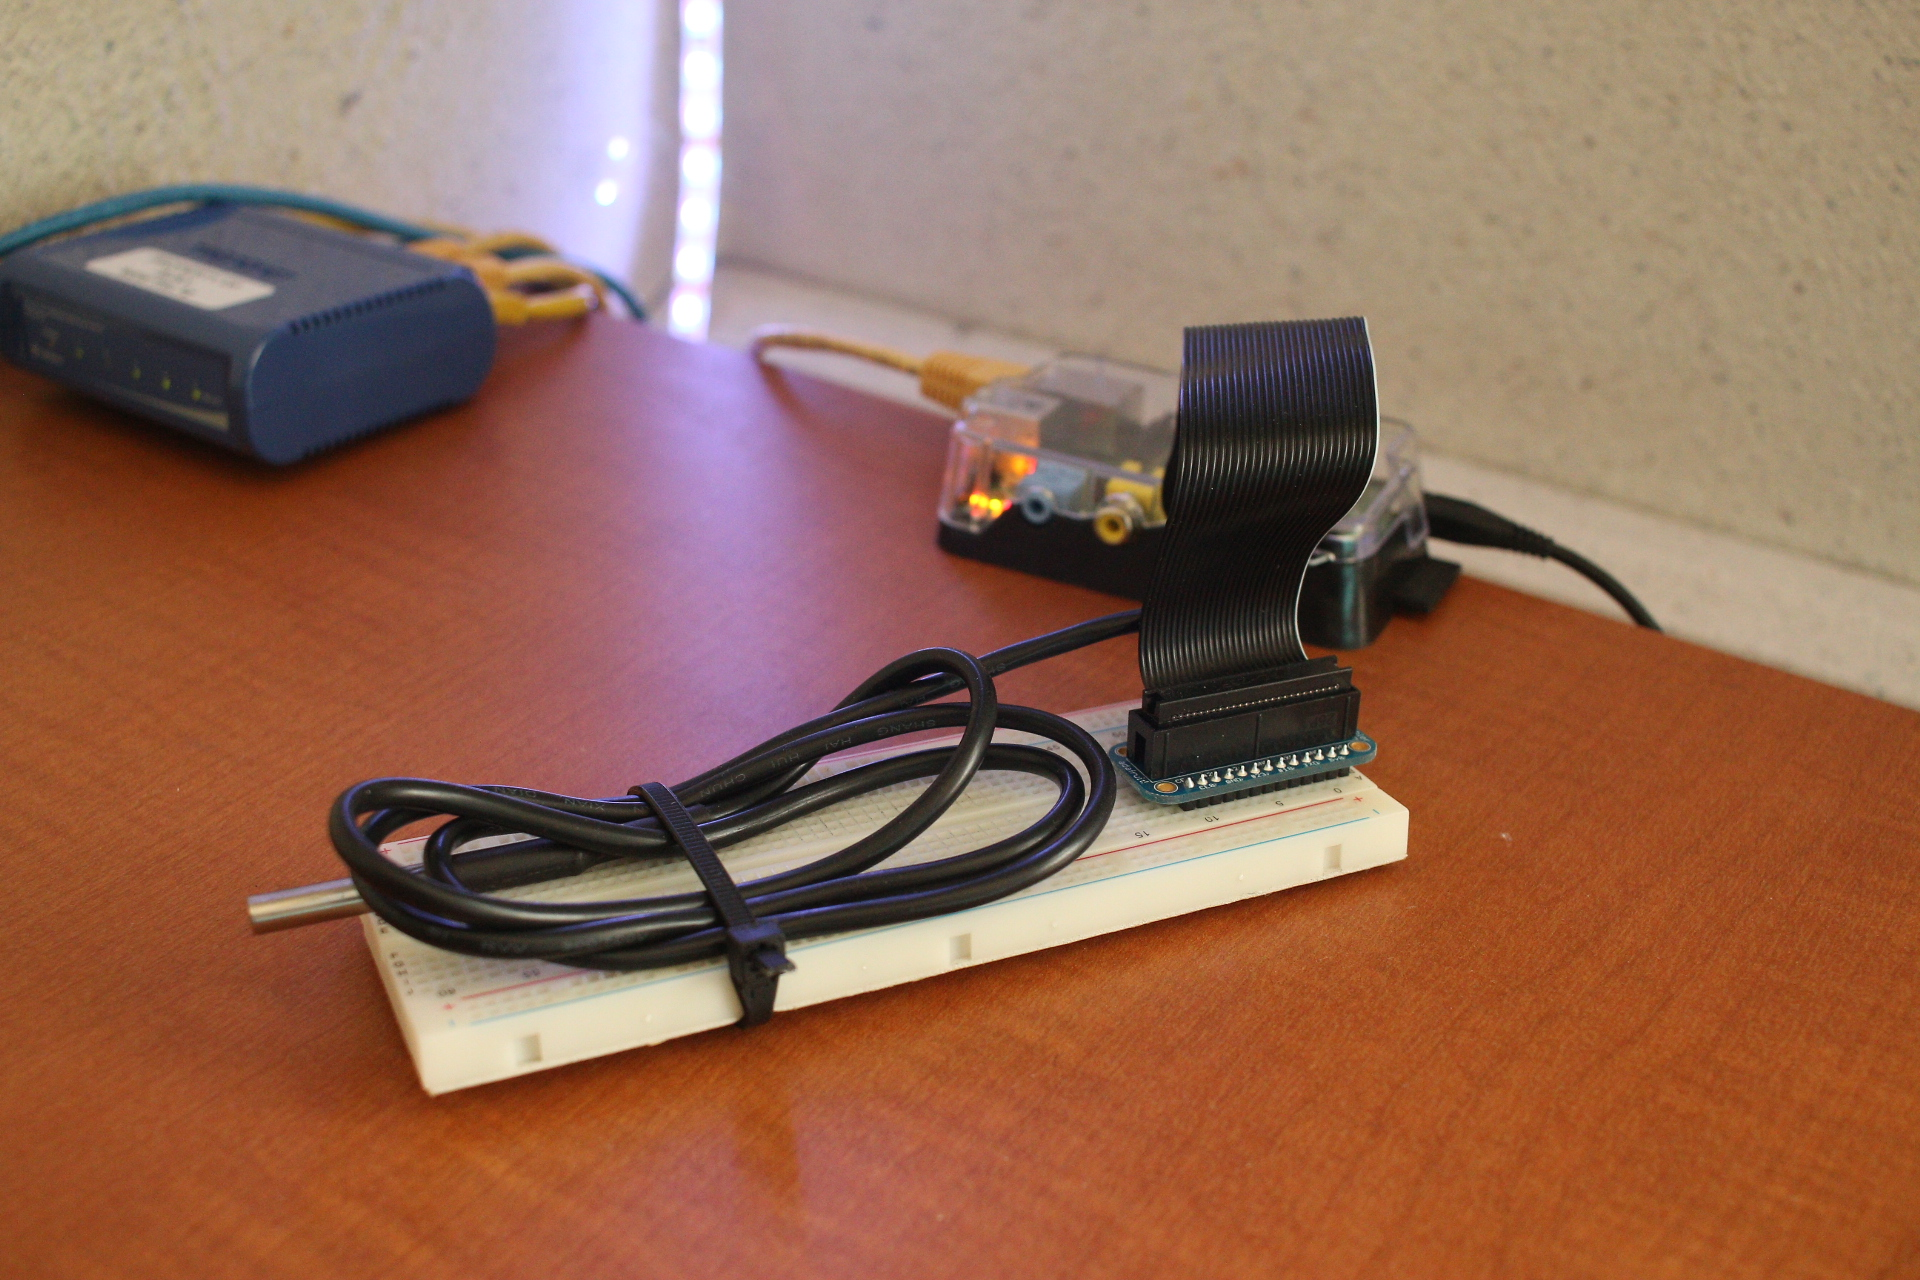
\includegraphics[scale=.15]{rpi.jpg}\\
			[1cm]
		\end{center}
		
		\begin{flushright}
			\textsc{\Large Brendan Lowe\\
				Cesar Done\\
				Heidi Fritz\\
				Jabari Dash\\
				Roberto Milanese\\
				Victoria Bottali\\}
		\end{flushright}
	\end{titlepage}
	
%====================================================================================================================================
	\tableofcontents
%====================================================================================================================================
	
	\newpage	
	\section{Introduction}\label{sec:intro}
		This report documents the process that several students in Dr. Chirakkal Easwaran's Spring 2016
		Embedded Linux class took to complete their final class project. The course is designed to introduce students to 
		the fundamentals of Linux programming - particularly embedded Linux. Dr. Easwaran's course is oriented around the Raspberry Pi
		and the Raspbian (Debian) Linux distribution to give students this fundamental practice. Students throughout the 	
		course learn basic terminal commands, how to read temperature sensors, how write to a SQLite3 database, and more. Midway 
		through the semester, students are separated into groups, and assigned a final project. Students Brendan Lowe, Cesar 
		Done, Heidi Fritz, Jabari Dash, Roberto Milanese, and Victoria Bottali were tasked with collecting 
		temperature data throughout Bliss Hall at the SUNY New Paltz campus and representing it graphically
		for later analysis by the Sustainability Office.                                                                                                                                                                                                                                                                                                                                                                                                                                                                                                                                                                                                                                                                                                                                                                                                                                                                                                                                                                                                                                                                                                                                                                                                                                                                                                                                                                                                                                                                                                                                                                                                                                                                                                                                                                                                                                                                                                                                                                                                                                                                                                                                                                                                                                                                                                                                                                                                                                                                                                                                                                                                                                                                                                                                                                                                                                                                                                                                                                                                                                                                                                                                                                                                                                                                                                                                                                                                                                                                                                                                                                                                                                                                                                                                                                                                                                                                                                                                                                                                                                                                                                                               
		
%====================================================================================================================================
		
	\newpage
	\section{Individual Student Responsibilities}\label{sec:responsibilities}
		\begin{minipage}{0.45\textwidth}
			\begin{itemize}[label={}]
  				\item
  					\begin{figure}[H]
  						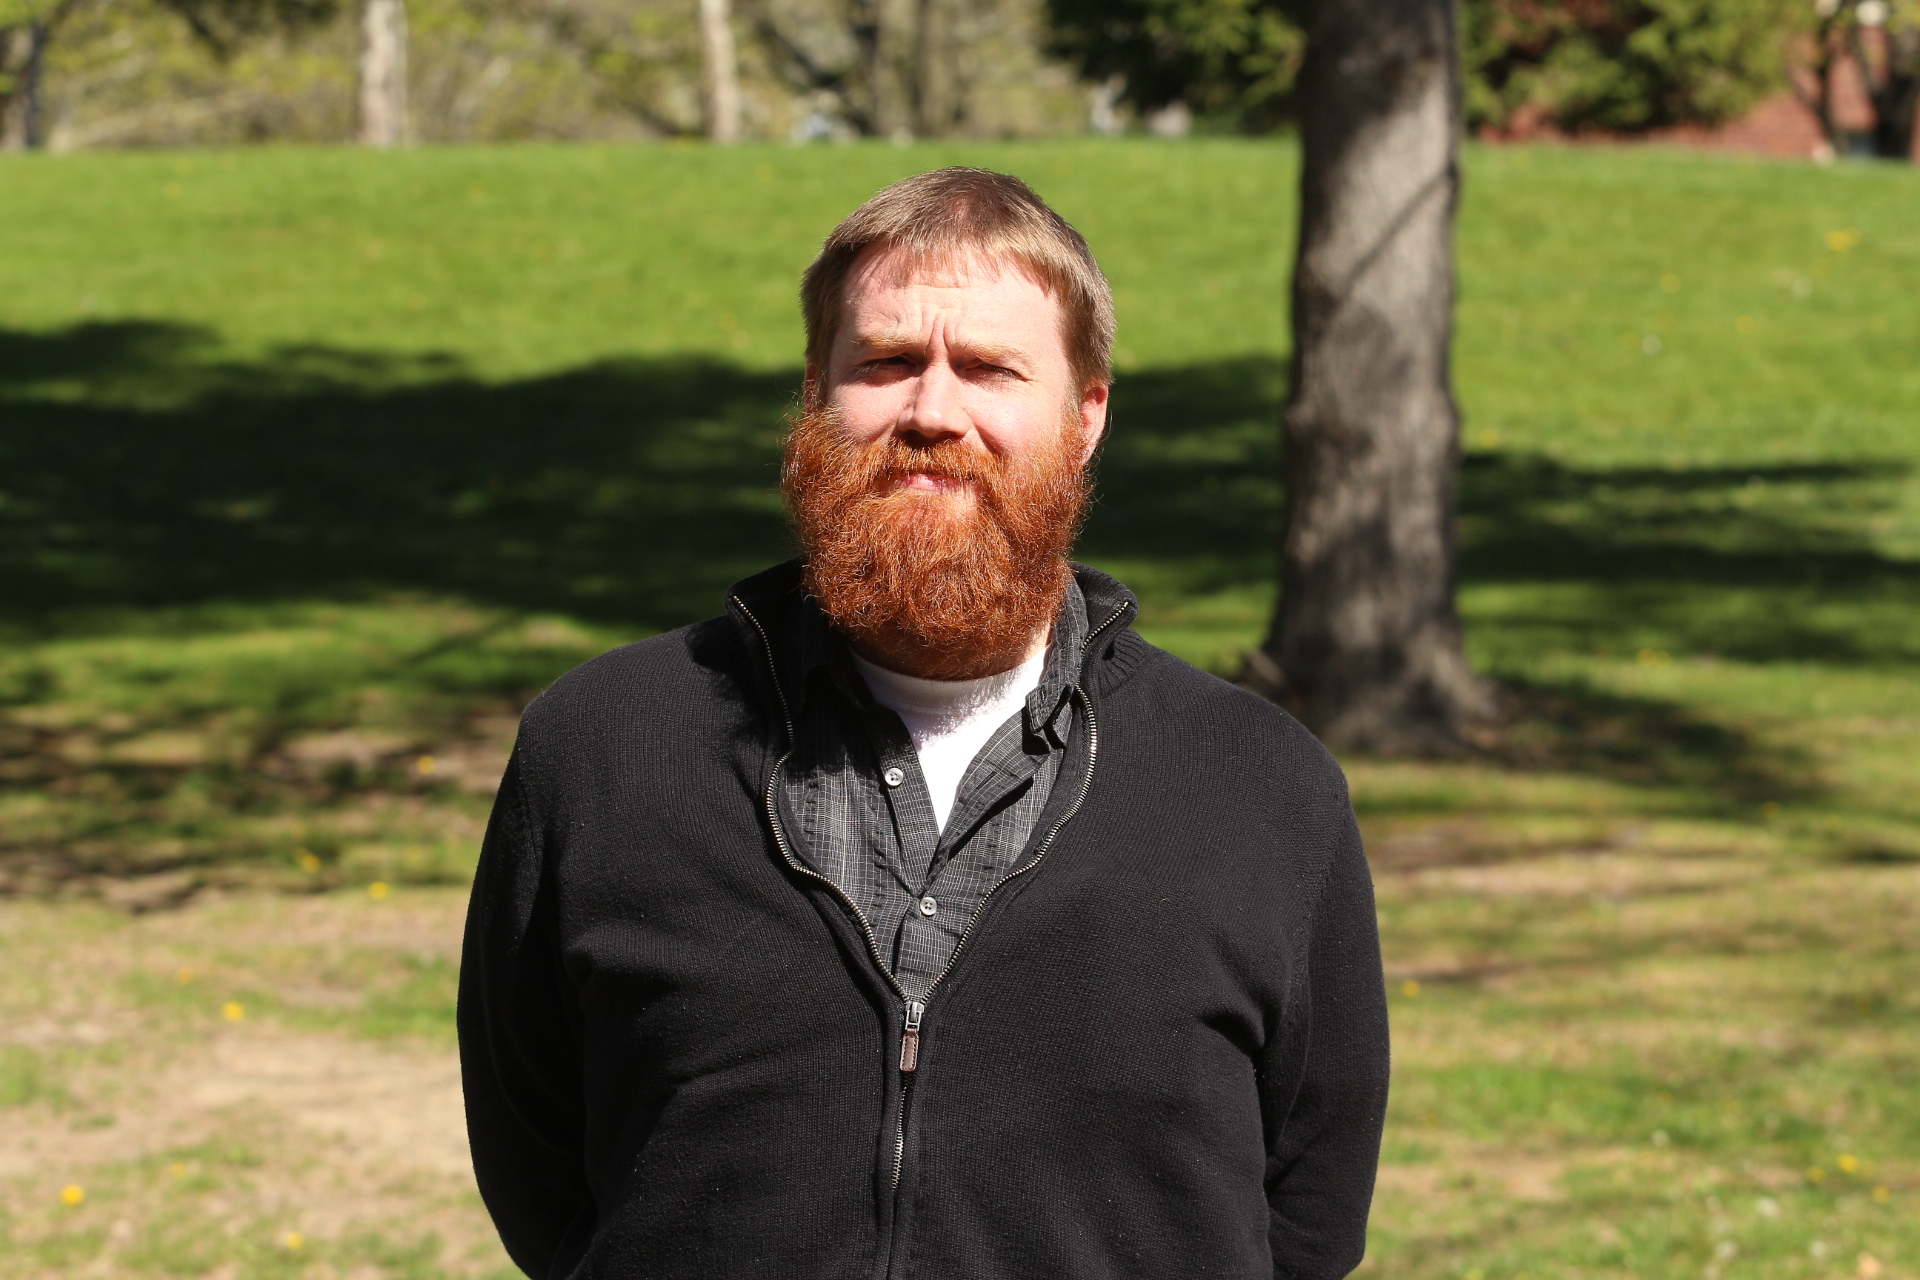
\includegraphics[scale=.07]{brendan.jpg}\\
  							\captionsetup{labelformat=empty}
  							\caption{Brendan handled server-side programming, networking, deployment}
  					\end{figure}
  				\item
  					\begin{figure}[H]
  						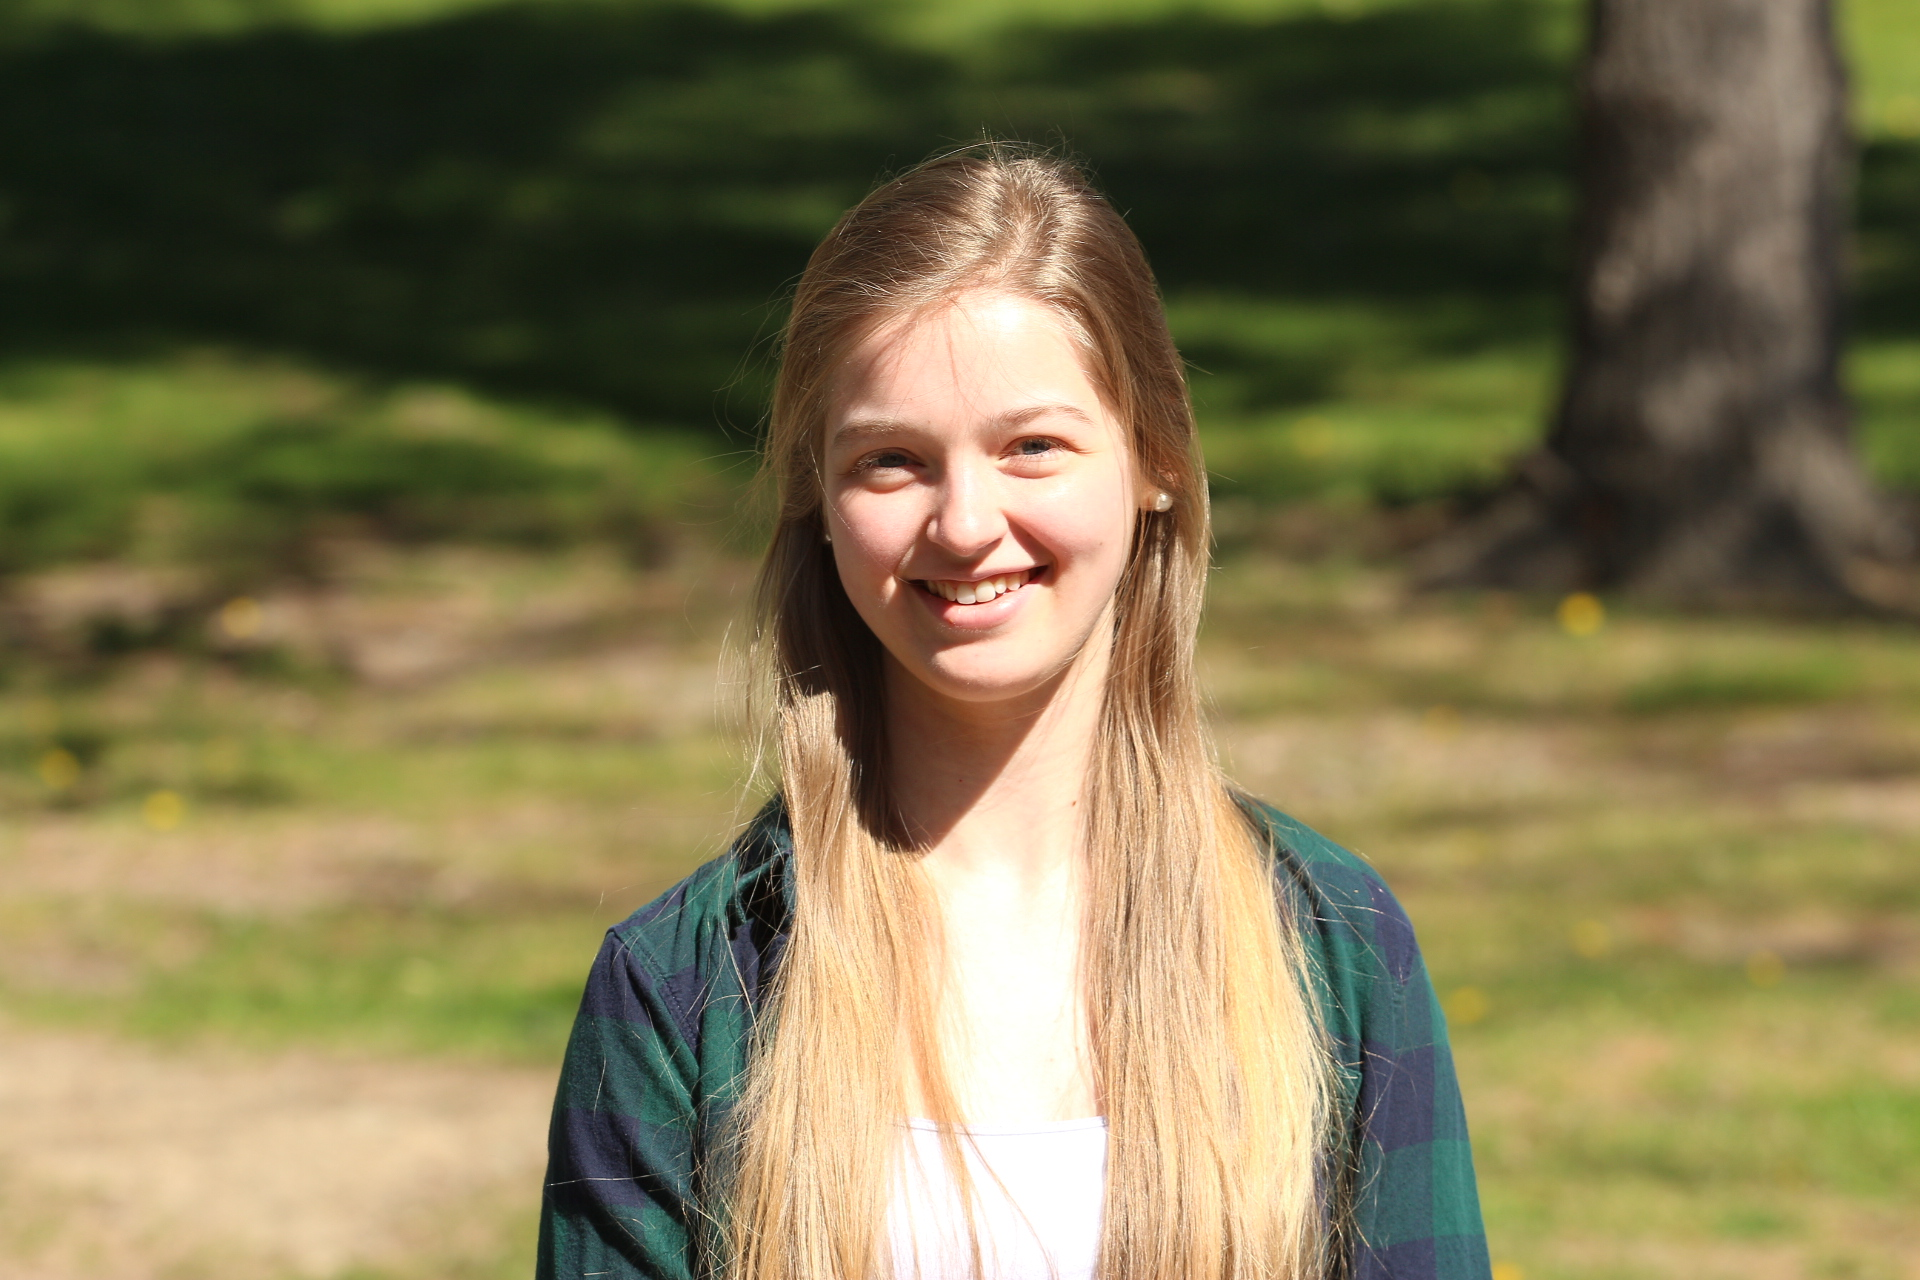
\includegraphics[scale=.07]{heidi.jpg}\\
  							\captionsetup{labelformat=empty}
  							\caption{Heidi handled  client-side programming, front-end programming
  										}
  					\end{figure}
  				\item
  					\begin{figure}[H]
  						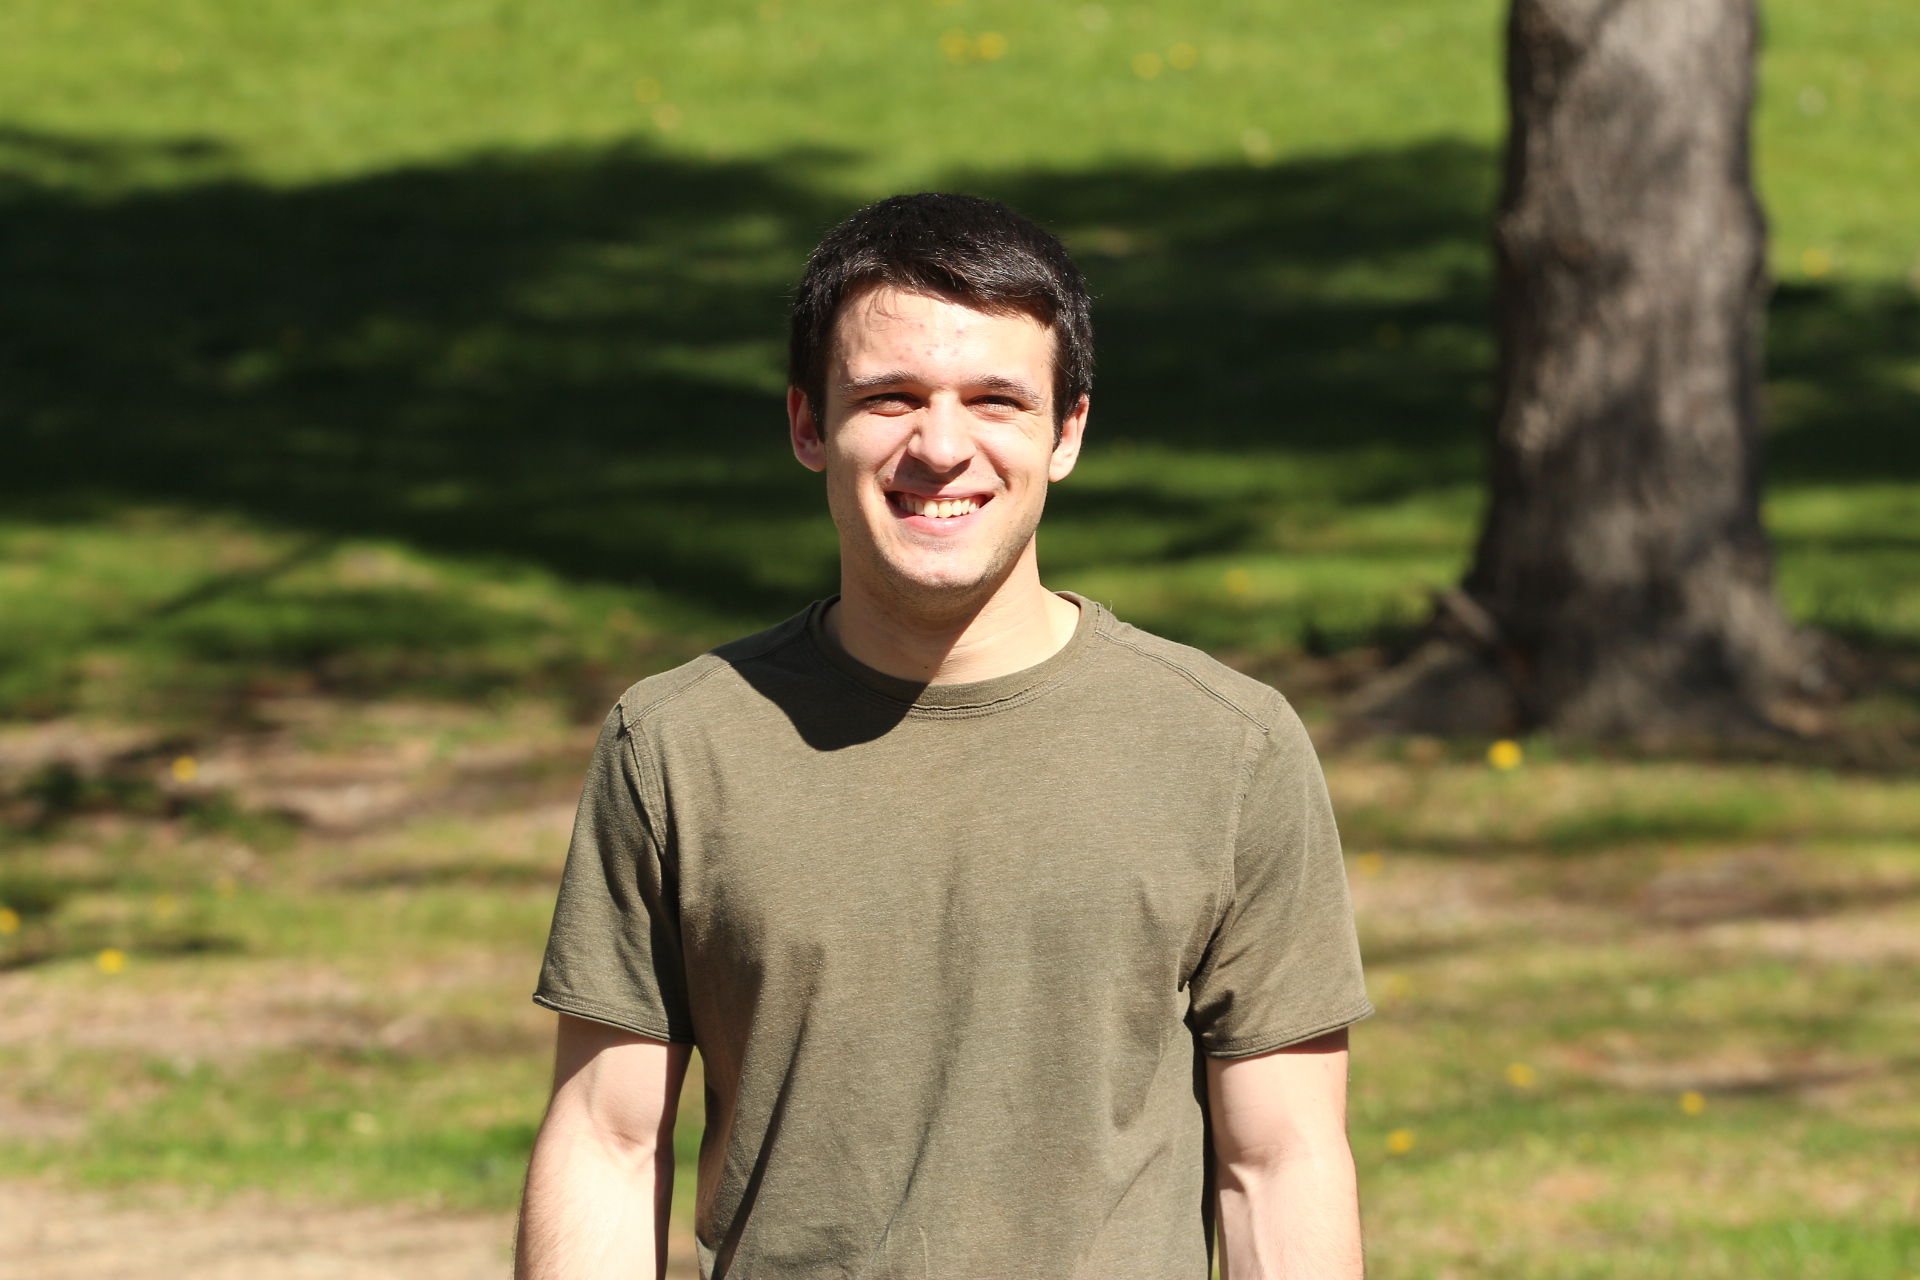
\includegraphics[scale=.07]{roberto.jpg}\\
  							\captionsetup{labelformat=empty}
  							\caption{Roberto handled front-end programming, GUI design}
  					\end{figure}
			\end{itemize}
		\end{minipage}
		\hfill
		\begin{minipage}{0.45\textwidth}
			\begin{itemize}[label={}]
				\item
  					\begin{figure}[H]
  						
\includegraphics[scale=.07]{cesar.jpg}\\
  							\captionsetup{labelformat=empty}
  							\caption{Cesar handled front-end programming, GUI design}
  					\end{figure}
  				\item
  					\begin{figure}[H]
  						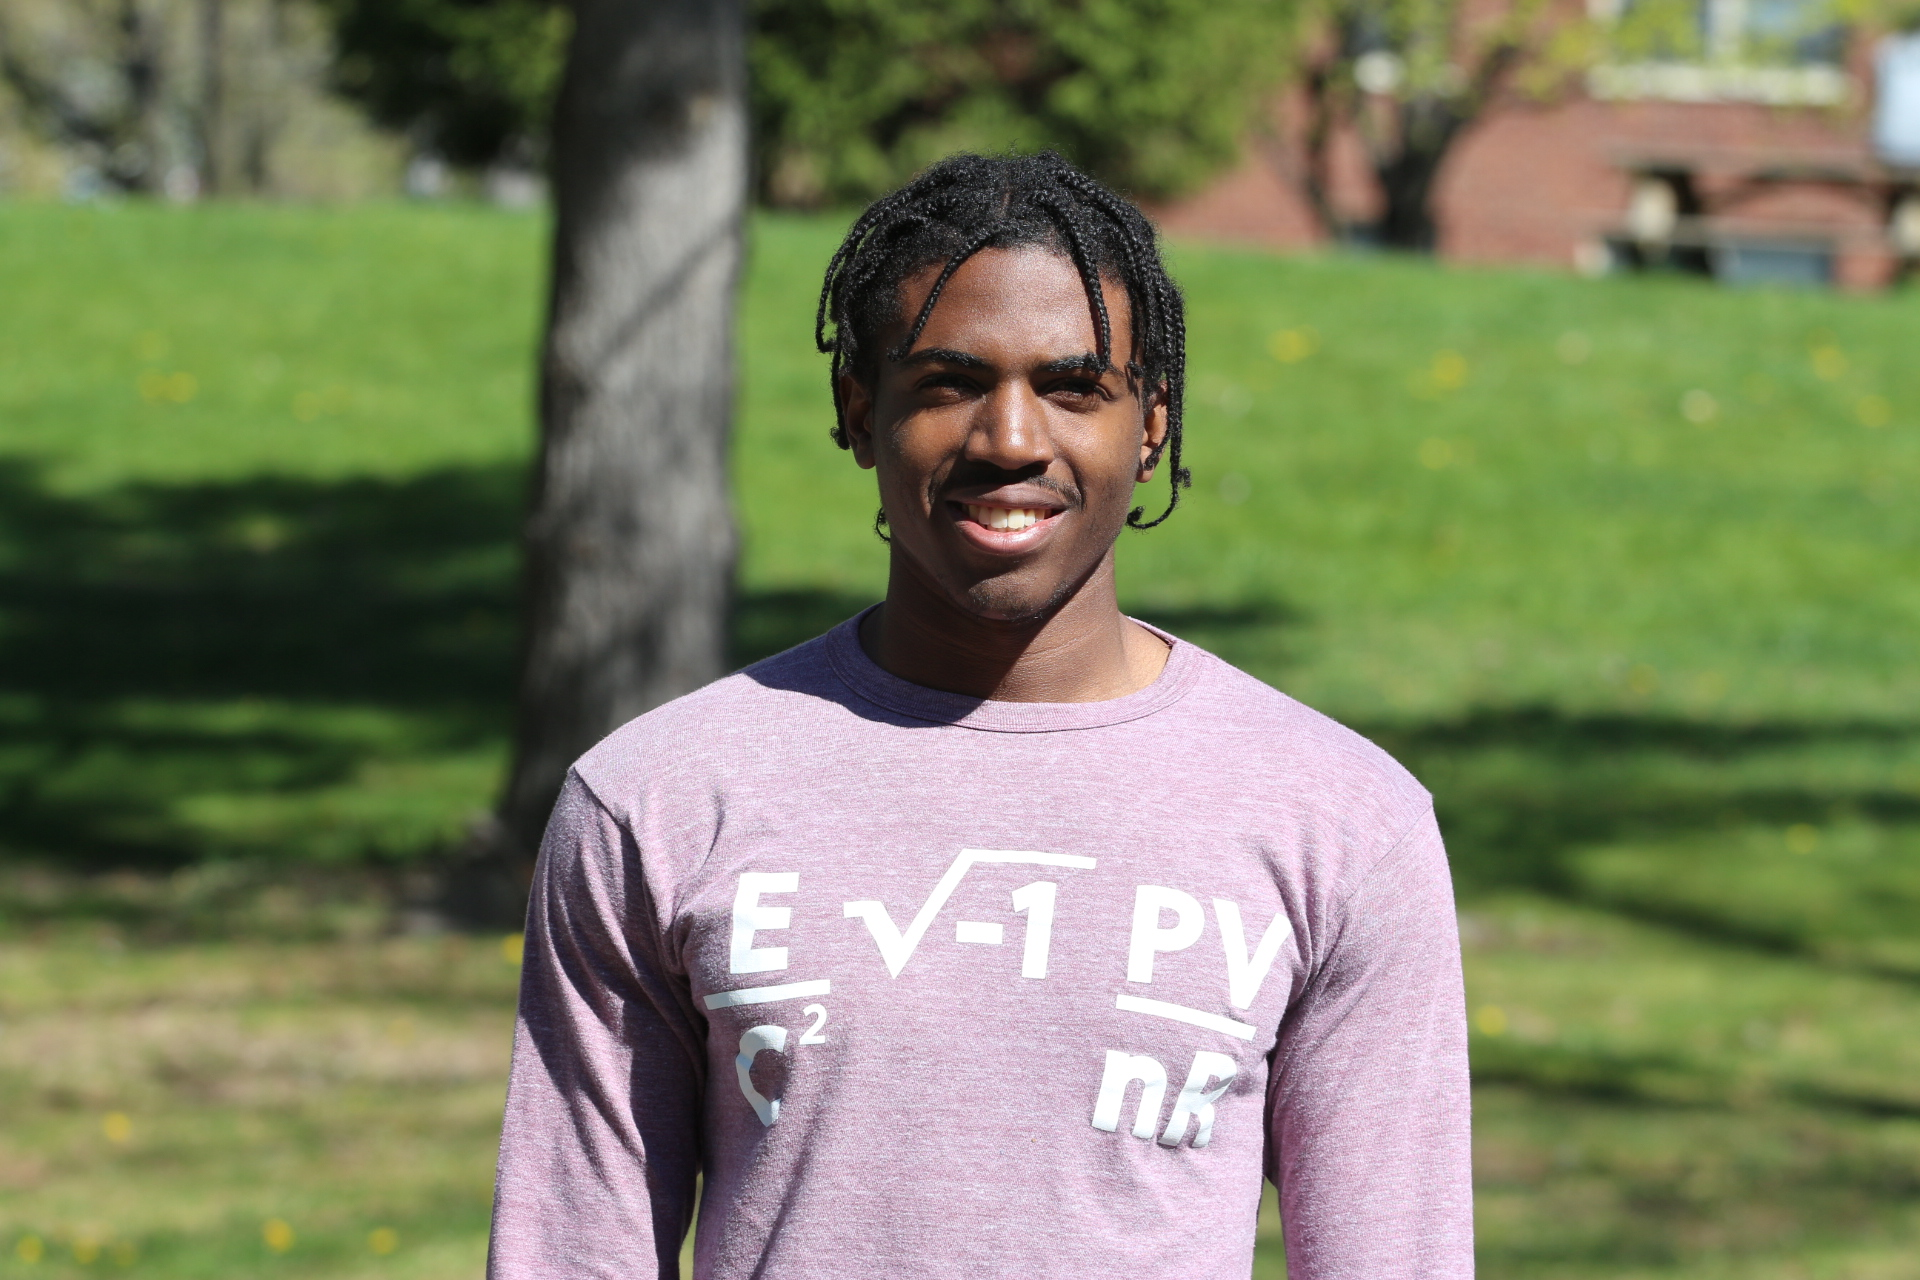
\includegraphics[scale=.07]{jabari.jpg}\\
  							\captionsetup{labelformat=empty}
  							\caption{Jabari handled documentation, logistics, GUI design}
  					\end{figure}
  				\item
  					\begin{figure}[H]
  						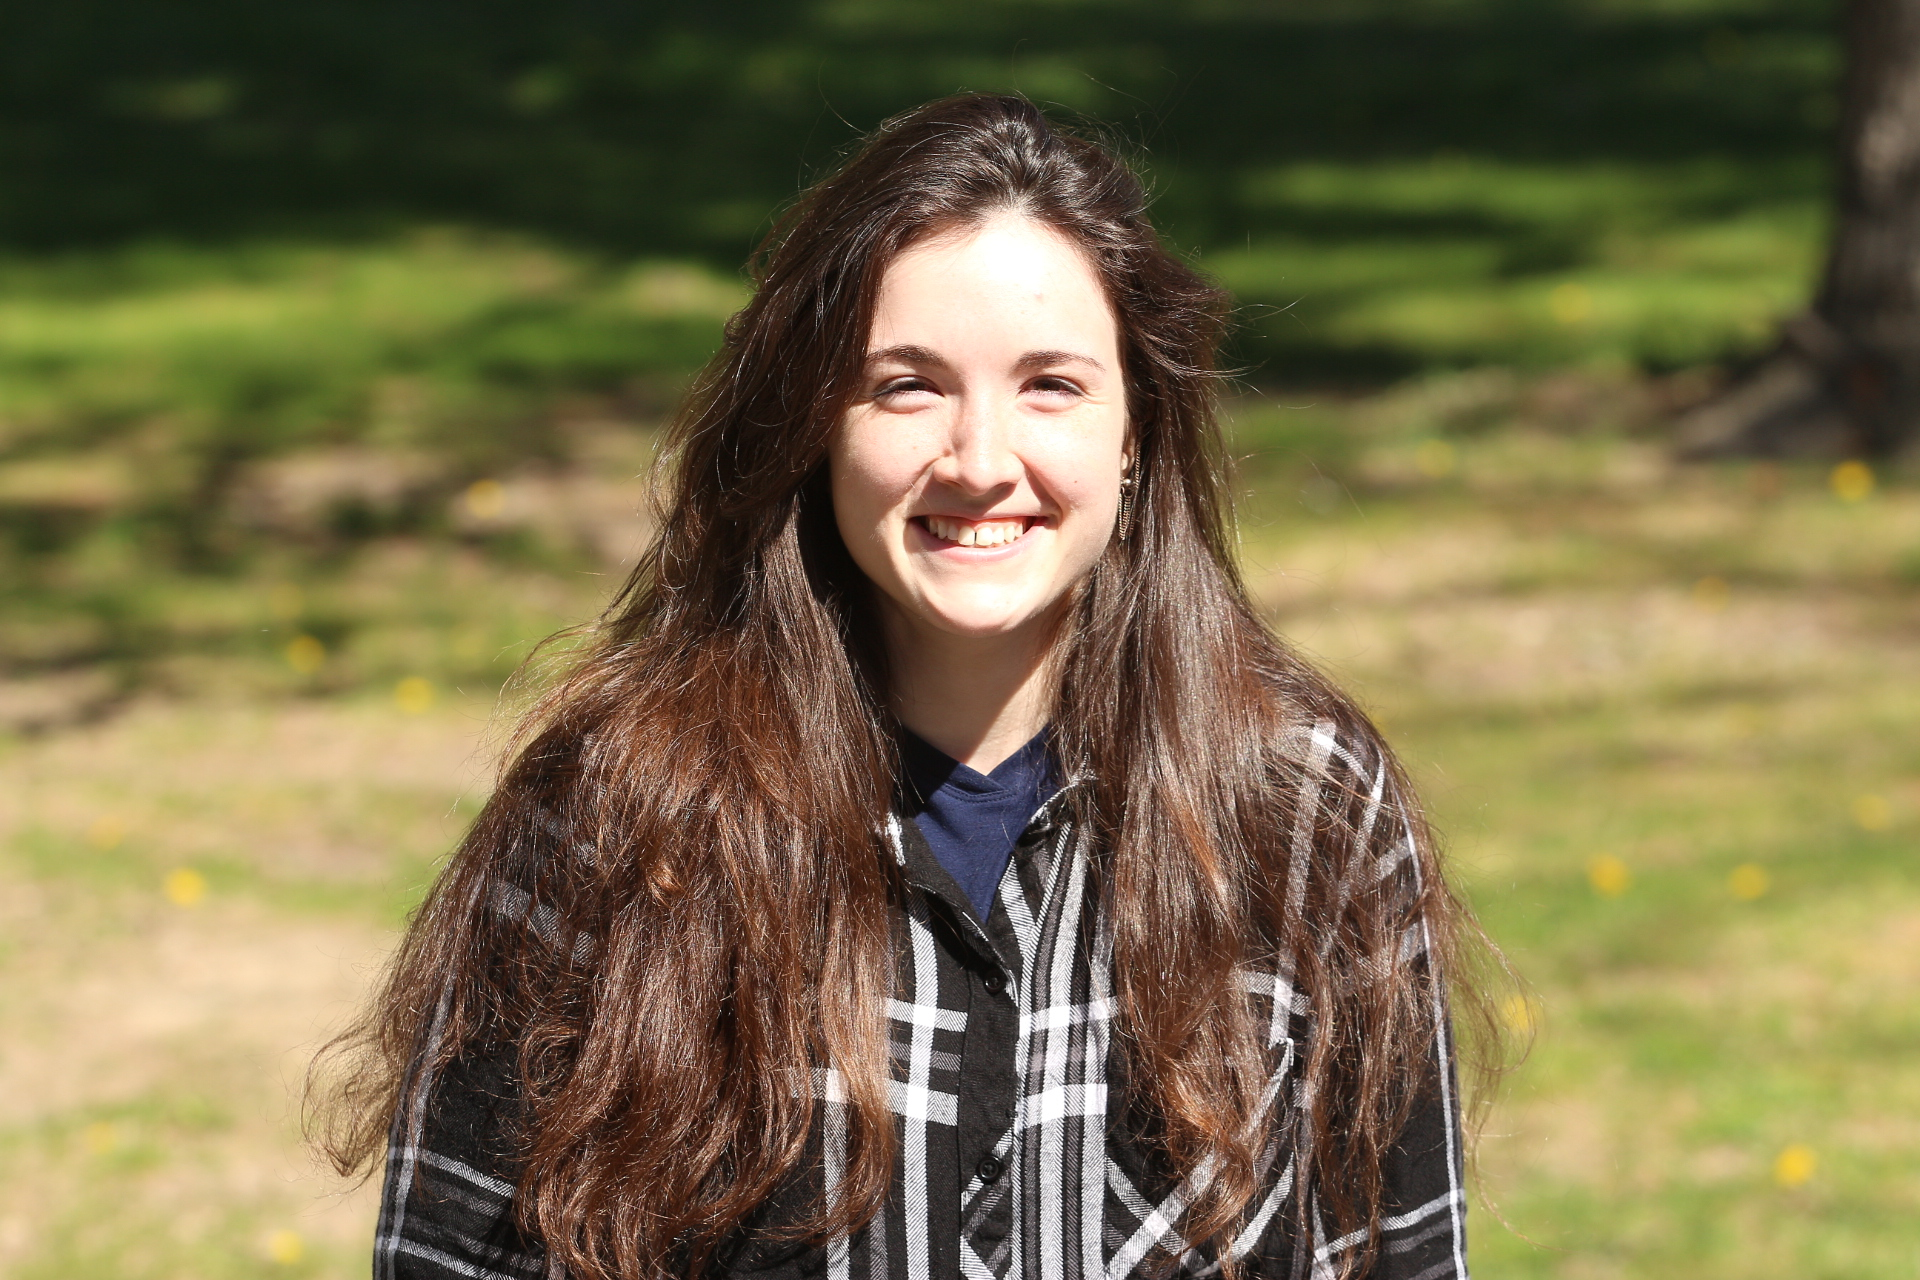
\includegraphics[scale=.07]{victoria.jpg}\\
  							\captionsetup{labelformat=empty}
  							\caption {Victoria handled client-side programming}
  					\end{figure}
			\end{itemize}
		\end{minipage}%
		
%====================================================================================================================================
	
	\newpage
	\section{Project Goals}\label{sec:goals}
		\subsection{Student Learning Outcome Goals}
			For this project students will be provided with first hand experience with software engineering. Being a Software
			Engineer / Developer is different than simply being a Coder or Programmer. A Programmer is someone who knows a set 
			of programming languages, and knows how to write programs as assigned in those languages - the same for a coder. 
			A Software Developer differs in that they analyze a problem, gather a team, and design and implement a solution. 
			The goal of this project is just that. The task of this project is to familiarize students with processes
			and resources that Software Engineers use when creating solutions.
			
			For this given project, students will use resources such as GitHub as a repository for their code. Using GitHub will
			give students the opportunity to work collaboratively, stage, and commit code. They will write software using 
			Python, JavaScript, PHP, SQLite3, MySQL, HTML, and more. They will also obtain some of the soft skills required such
			as team work, communication, and basic negotiation skills (in terms of decision making).
		\subsection{Project Output Goals}
			To have several weeks worth of temperature data on Bliss Hall accessible in a user friendly web page that the
			Sustainability Officer will be able to view and later analyze.\\	
		
		\begin{figure}[H]
  			\begin{center}	
				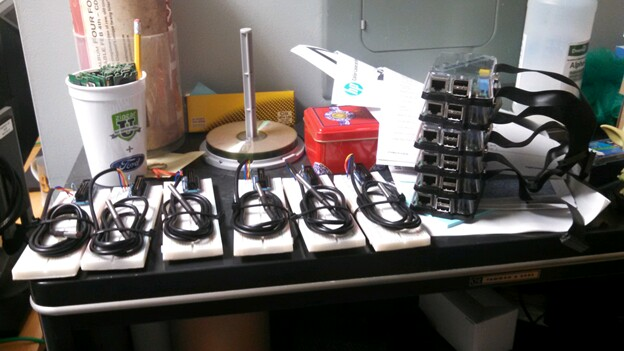
\includegraphics[scale=.5]{pre_deployment.jpg}
			\end{center}
  				\captionsetup{labelformat=empty}
  				\caption{6 Raspberry Pis at the pre-deployment stage}
  		\end{figure}			
			
%====================================================================================================================================
		
	\newpage	
	\section{Materials \& Programming Languages}\label{sec:materials}
		\subsection{Hardware}
			\begin{itemize}
				\item Raspberry Pi Single Board Computer (8)
				\item Adafruit Raspberry Pi Enclosure(8)
				\item MicroUSB + Wall Adapter Kit (8)
				\item 4GB+ SD Card (8)
				\item Cobbler Cable + Pi Header Kit (8)
				\item DS18B20 Digital Temperature Sensor (8)
				\item Breadboards (8)
				\item 4.7k Ohm Resistor (8)
				\item Ethernet Cables (9)
				\item Networking Switch (1)
				\item Wire Tie (8)
				\item Duct Tape
			\end{itemize}
			
		\subsection{Software}
			\subsubsection{Client-Side Programming}
				\begin{itemize}
					\item Python
					\item SQLite3
				\end{itemize}	
			\subsubsection{Server-Side Programming}
				\begin{itemize}
					\item JavaScript
					\item PHP
					\item HTML
					\item MySQL
				\end{itemize}
			\subsubsection{Other}
				\begin{itemize}
					\item Crontab
					\item GitHub
					\item LATEX
				\end{itemize}
		
%====================================================================================================================================
			
	\newpage
	\section{Implementation}\label{sec:implementation}
		\subsection{Overall Structure}
			Students distributed several internet connected Raspberry Pi computers throughout Bliss Hall in residents' rooms
			where each Pi periodically reads the current ambient temperature in the room and writes it to a local database. A 
			Linux Apache MySQL and PHP (LAMP) server running on SUNY New Paltz servers periodically performs a pull request on
			each Pi, and compiles all of the temperature data in a MySQL database.
			
			\begin{figure} [H]
				\begin{center}
					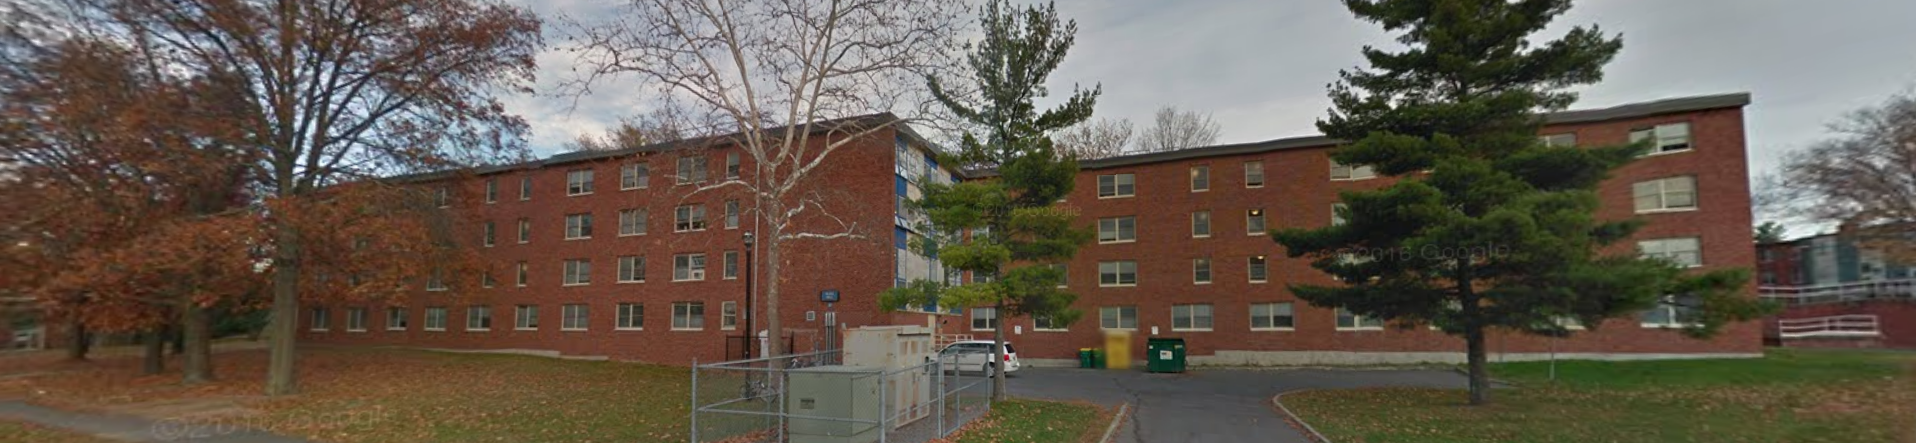
\includegraphics[scale=.3]{bliss.png}
						\captionsetup{labelformat=empty}
						\caption{Google Maps screen-shot of rear of Bliss that demonstrates Raspberry Pi / Sensor distribution}
				\end{center}
			\end{figure}
			
%------------------------------------------------------------------------------------------------------------------------------------
			
	\newpage
			
		\subsection{Temperature Sensor Setup}	
			The temperature sensor is connected to the Raspberry Pi's General Purpose Input Output (GPIO) pins via breadboard, 
			and the 24-pin cobbler cable. The DS18B20 has three cables: ground (GND), 3.0 volt - 5.0 volt power line, and a data line. 
			We connect the GND to and GND pin on the Raspberry Pi, the power line to the 3.3v rail, and the data line to GPIO \#4.
		 	We then set up a pull-up resistor that connects the data line (pin 4) to the 3.3v line.
							
				\begin{figure}[H]
  					\begin{center}	
						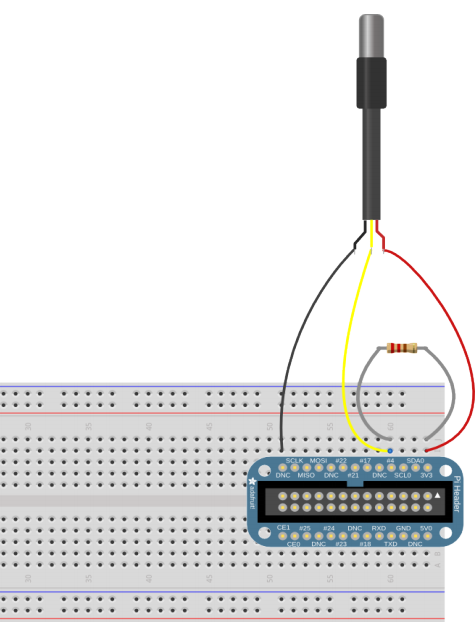
\includegraphics[scale=.8]{breadboard.png}\\
					\end{center}
  						\captionsetup{labelformat=empty}
  						\caption{DS18B20 Digital Temperature Sensor connected to the breadboard using a  4.7k pull-up resistor}
  				\end{figure}	
  				
%------------------------------------------------------------------------------------------------------------------------------------  	
  	
  	\newpage					
		
		\subsection{Client-Side Software (Raspberry Pi)}
			Each Pi will have 3 Python scripts that allow the Pi to collect data, convert it to JavaScript Object
			Notation (JSON) format, and return the JSON to the LAMP server.
			
			\subsubsection{Python Scripts}
				\begin{itemize}
					\item tempLog.py: Creates a Cronjob (scheduled task) the first time tempLog.py executes. The Cronjob executes tempLog.py every 10 minutes. 
					The script reads the ambient temperature
					in celcius and writes it to a SQLite3 database file called climate\_info.db
						\begin{center}
							\includegraphics[scale=.4]{tempLogFlowchart.png}\\
						\end{center}
					\item index.py: When passed a given start and stop date, index.py sets up a Flask server on the Pi and 
									converts the data from the SQLite database into JSON objects. The JSON is put onto the Flask server in
									preparation to be sent to the LAMP server.
					\item json\_push.py: Creates the JSON post to push to data to the LAMP server.
				\end{itemize}
				
			\subsubsection{SQLite3 Database Schema}	
				
%------------------------------------------------------------------------------------------------------------------------------------
			
	\newpage		
			
		\subsection{Server-Side Software (LAMP Server)}
			INSERT OVERVIEW HERE
			\subsubsection{PHP Scripts}
			\subsubsection{MySQL Database Schema}
			\subsubsection{Graphical User Interface}
		
%====================================================================================================================================		
	\newpage
	\section{Student Analysis}\label{sec:analysis}
		\subsection{As of April 25, 2016}
			\begin{itemize}
				\item Brendan Lowe:
				\item Cesar Done: The project thus far has been running very smoothly. We are lucky to have access to several rooms here on campus as well 
								  as several network settings that students don’t regularly have. The Pi’s haven’t given us any problems and the actual set 
								  up and maintenance of them have been smooth as well. This project can  become a even bigger, funded project by the school
								   if we manage to provide accurate as well as beneficial data to the school. Also if we can create a simple interface that 
								   school can use to access the data, they would be more inclined to support and provide their services for the project. 
							
				
				\item Heidi Fritz: This project had simple tasks that we planned out and I took on the back end operations that the raspberry pi would 
				carry out to collect the temperature and humidity data.  To do this I connected my own temperature sensor to a personal pi and wrote 
				python script which consisted of four functions.  A function to get the temperature from the device, log the temperature and time into a 
				sqlite database, create a cronjob to repeat data collection, and a main function to start the process.  One struggle I came across was 
				opening the device file so it would work on every pi.  I imported glob to find the correct path name within the pi.  The python script 
				was easily integrated with the other scripts to work on one pi so we could make copies of the sd card.  In the end, I met the team goals 
				and expectations.
				\item Jabari Dash: The project so far is going well in that the data is being collected correctly.
									The beginning was challenging in that the group was lost because we were unsure of how to 
									implement this project - particularly the intercommunication between the 
									Raspberry Pis and the server. We wanted to used static IP addresses on the 
									school network, but this was not permitted. Fortunately, Brendan's skill in networking,
									and more importantly, his position as the Networking Manager allowed us to have a subnet
									on the school network, with static IP addresses. This was a "quick and dirty" solution that 
									allowed us to focus more on other elements of the projects, but also reduces the scalability
									and portability of our implementation.
				\item Roberto Milanese:
				\item Victoria Bottali:	My goal for the end of the project is to have a working Flask app that is able to graph 
										the temperature from the back-end based on different sets of parameters passed via user input. More 				
										specifically, I would like the app to be able to dynamically plot data given a broad spectrum of 
										options,including different periods of time and whether or not the user would like to see multiple data sets 
										plotted together for comparison. I think the project turned out well, though we needed 
										to rely on a a few "quick" fixes here and there in the interest of time.   	
			\end{itemize}
			
			\subsection{As of May 1, 2016}
				\begin{itemize}
					\item Brendan Lowe:
					\item Cesar Done:
					\item Heidi Fritz:
					\item Jabari Dash:
					\item Roberto Milanese:
					\item Victoria Bottali:			
				\end{itemize}
			
%============================================================================================================================			
	\newpage
	\section{Conclusion}\label{sec:conclusion}

\end{document}